\section{Final Convolutional Neural Network}\label{sec:cnnfinalcnn}

The final CNN is shown in \lstref{lst:finalcnn} and available in the definition
file named \code{cnndef.m}.

\lstinputlisting[language={matlab}, label={lst:finalcnn},
style={Matlab-editor}, basicstyle={\footnotesize\ttfamily}, caption={The final
CNN architecture and training options.}]{cnndef.m}

This network has been trained with 200 epochs. Samples were divided as follows:
\begin{itemize}
\item Training set: \(70\%\) (\(4200\) samples).
\item Validation set: \(15\%\) (\(900\) samples).
\item Test set: \(15\%\) (\(900\) samples).
\end{itemize}

A test set has been used since the validation set is used to select the output
network of the training process. So the test set allows for an unbiased
evaluation of the performance of the network.

Training ended after 3952 iterations (112 epochs plus some iterations), due to
validation loss not improving anymore. Complete results are shown in
\lstref{lst:cnnresults}. \figref{fig:cnnregression} shows the regression plots
for the CNN. The CNN clearly outperformed the MLP developed in \chref{ch:ecg}.

\lstinputlisting[language={}, label={lst:cnnresults},
caption={Results of the final Convolutional Neural Network.}]{cnnresults.txt}

\begin{figure}[htbp]
	\centering
	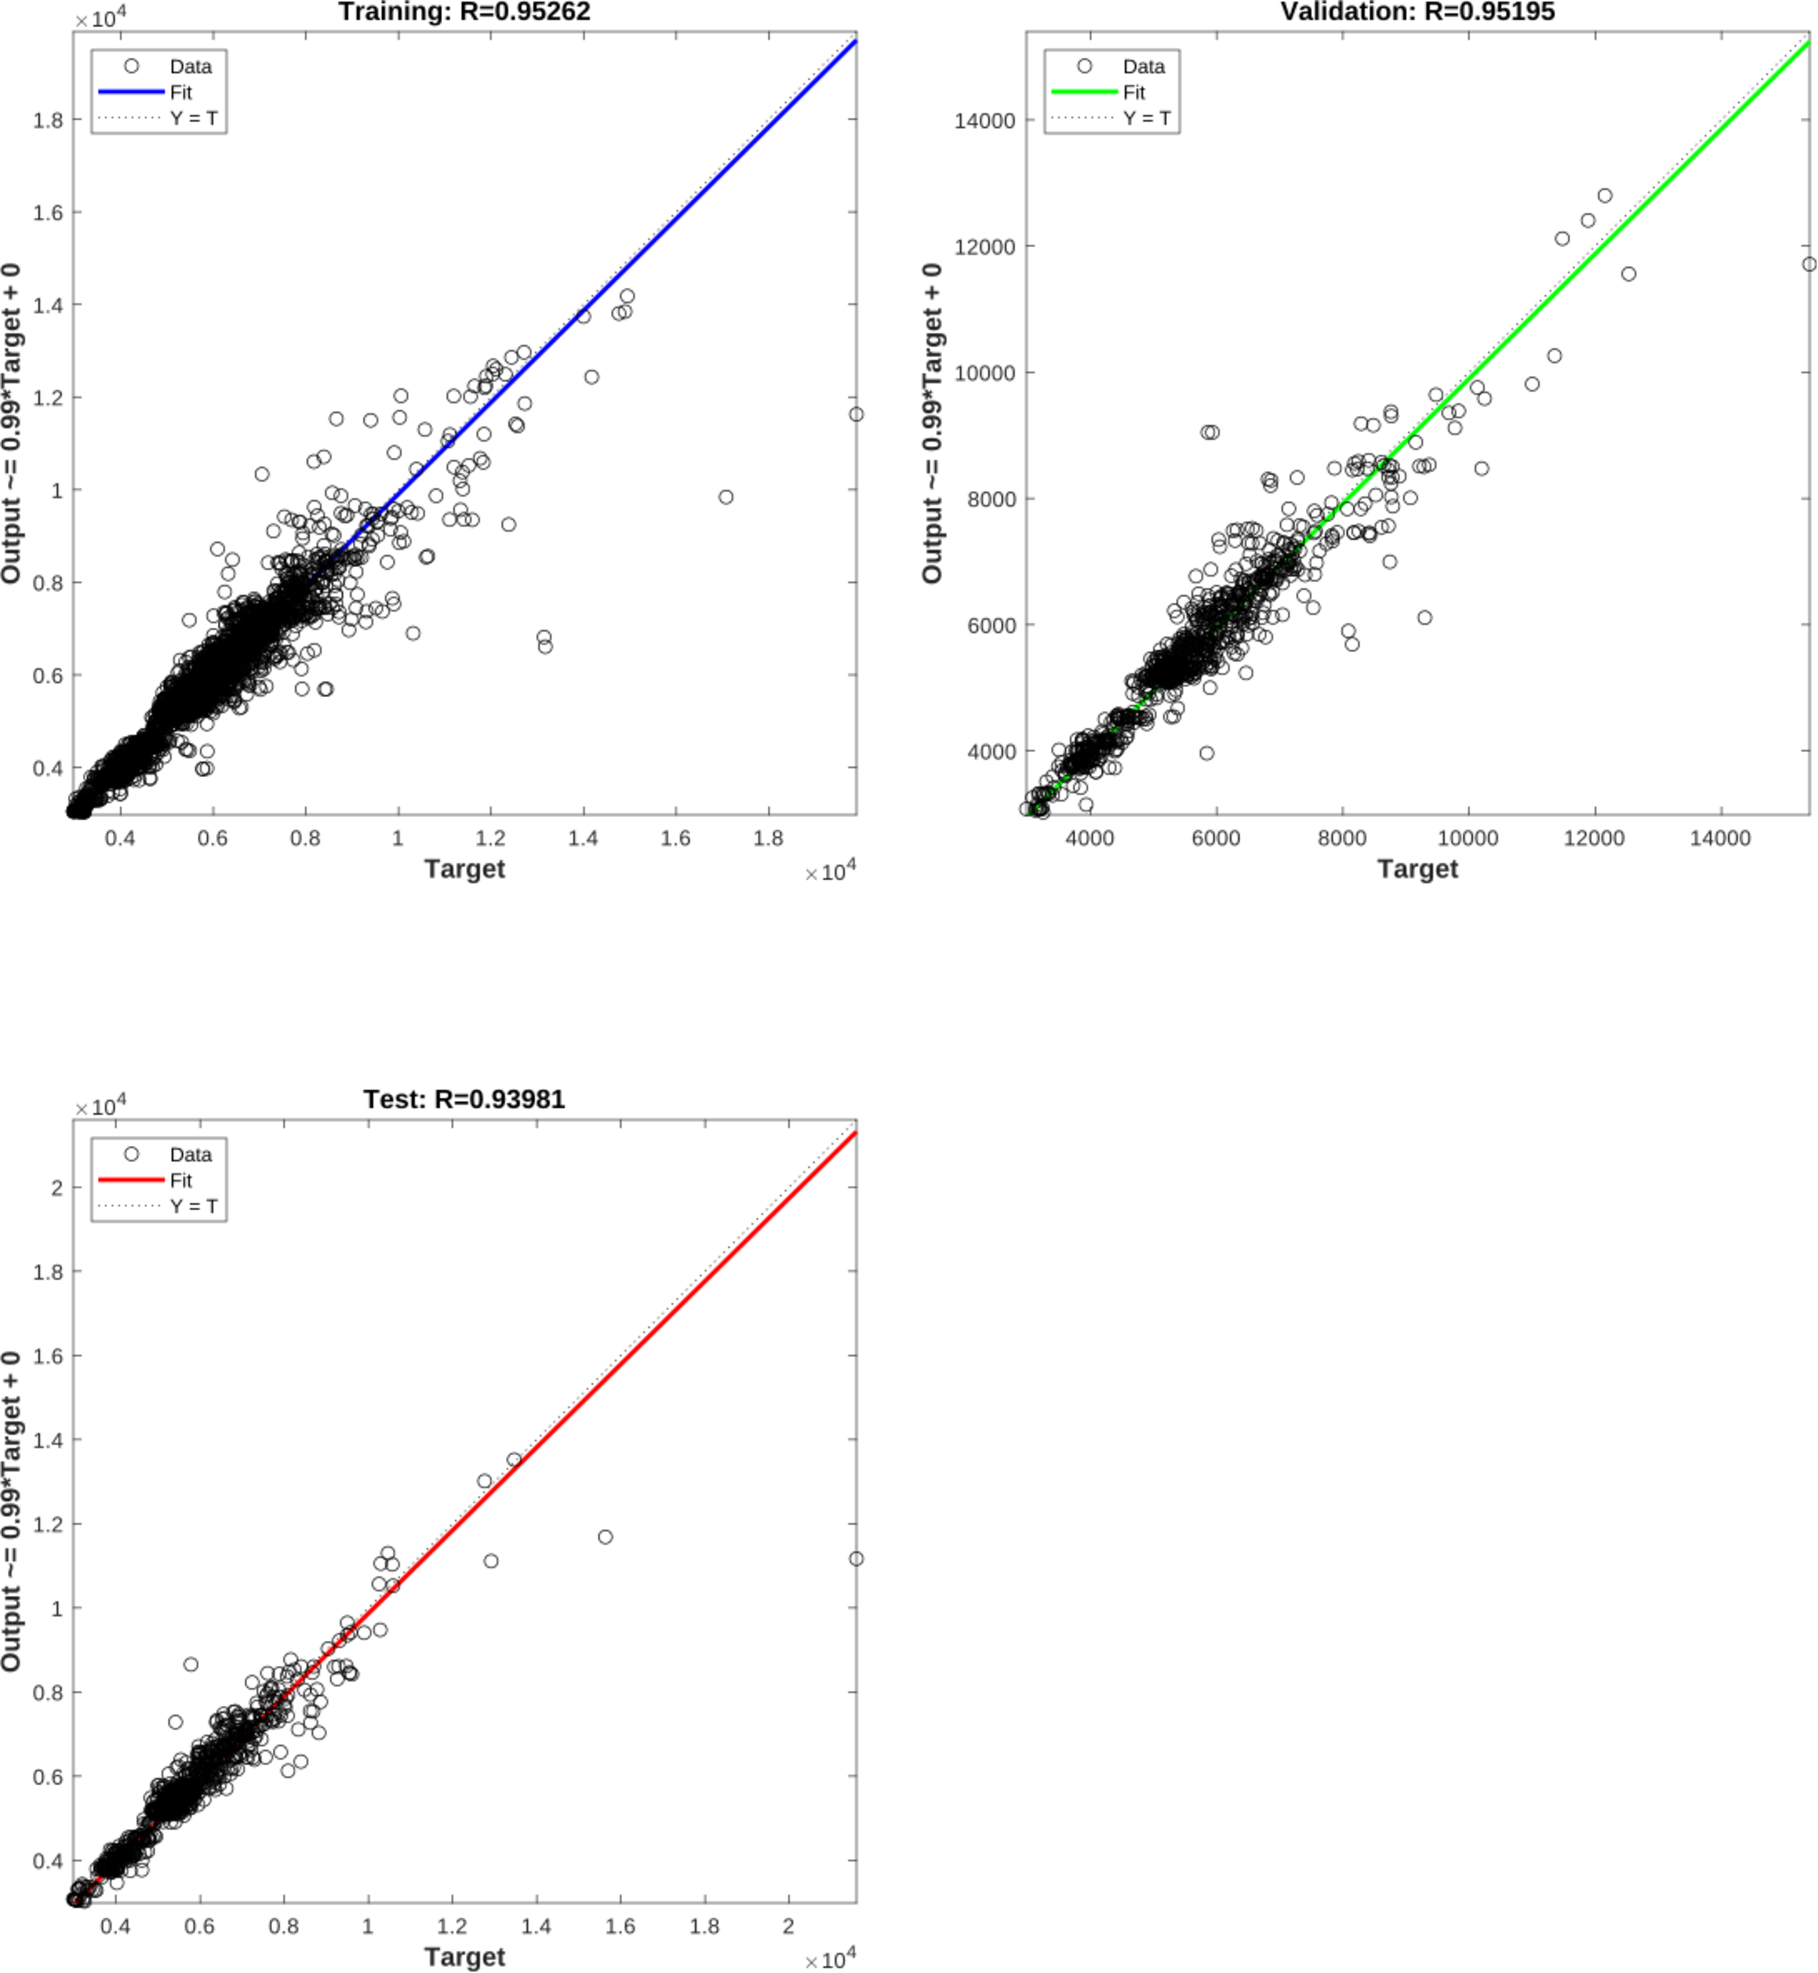
\includegraphics[width=\textwidth]{cnnregression}
	\caption{Regression plots for all three sets for the Convolutional
	Neural Network doing the task of estimating the ECG's standard
	deviation.}\label{fig:cnnregression}
\end{figure}
